\begin{tehtavasivu}

\begin{tehtava}
	Olkoot $A(x)$ avoin lause ''paikkakunnalla $x$ paistaa
	aurinko'' ja $T(x)$ avoin lause ''paikkakunnalla $x$
	tuulee''. Suomenna lause.
	\alakohdat{
	§ $\lnot T(x)$,
	§ $A(x) \land T(y)$,
	§ $\lnot A(\textrm{Lempäälä})$,
	§ $\lnot (A(\textrm{Turku}) \to T(\textrm{Kuopio}))$.
	}%
	\begin{vastaus}
		\alakohdat{
			§ Paikkakunnalla $x$ ei tuule.
			§ Paikkakunnalla $x$ paistaa aurinko ja paikkakunnalla $y$ tuulee.
			§ Lempäälässä ei paista aurinko.
			§ Turussa paistaa aurinko ja Kuopiossa ei tuule.
		}
	\end{vastaus}
\end{tehtava}

\begin{tehtava}
	Olkoot $S(x)$ avoin lause ''$x$ on suomalainen
	formulakuljettaja'' ja $E(x)$ avoin lause ''$x$ on
	eurooppalainen formulakuljettaja, joka ei ole
	suomalainen''. Kuljettaja voi olla joko nykyinen tai
	entinen. Ratkaise avoin lause, kun perusjoukko on
	$\{\textrm{Räikkönen}, \textrm{Vettel}, \textrm{Senna}\}$.
	\alakohdat{
	§ $S(x)$,
	§ $\lnot S(x)$,
	§ $E(x)$,
	§ $\lnot (S(x) \lor E(x))$.
	}%
	\begin{vastaus}
		\alakohdat{
			§ $\{\textrm{Räikkönen}\}$
			§ $\{\textrm{Vettel}, \textrm{Senna}\}$
			§ $\{\textrm{Vettel}\}$
			§ $\{\textrm{Senna}\}$
		}
	\end{vastaus}
\end{tehtava}

\begin{tehtava}
	Olkoon $Q(x)$ avoin lause ''$x^2 = 64$''. Onko lause a)
	$Q(-8)$ b) $Q(6)$ tosi?%
	\begin{vastaus}
		\alakohdat{
			§ On.
			§ Ei ole.
		}
	\end{vastaus}
\end{tehtava}

\begin{tehtava}
	Olkoon $P(x, y)$ avoin lause ''$x^2 + y \le 0$''. Onko
	lause a) $P(0, 0)$ b) $P(-1, 1)$ c) $P(5, -100)$ tosi?%
	\begin{vastaus}
		\alakohdat{
			§ On.
			§ Ei ole.
			§ On.
		}
	\end{vastaus}
\end{tehtava}

\begin{tehtava}
	Olkoot $S(x)$ avoin lause ''kuvio $x$ on symmetrinen
	jonkin suoran suhteen'' ja $P(x)$ avoin lause ''kuvio $x$
	on symmetrinen jonkin pisteen suhteen''. Perusjoukon
	muodostavat oheiset kuviot. Ratkaise avoin lause.
	\alakohdat{
	§ $S(x)$,
	§ $P(x)$,
	§ $\lnot (S(x) \lor P(x))$,
	§ $S(x) \lequiv P(x)$.
	}%
	\begin{center}
	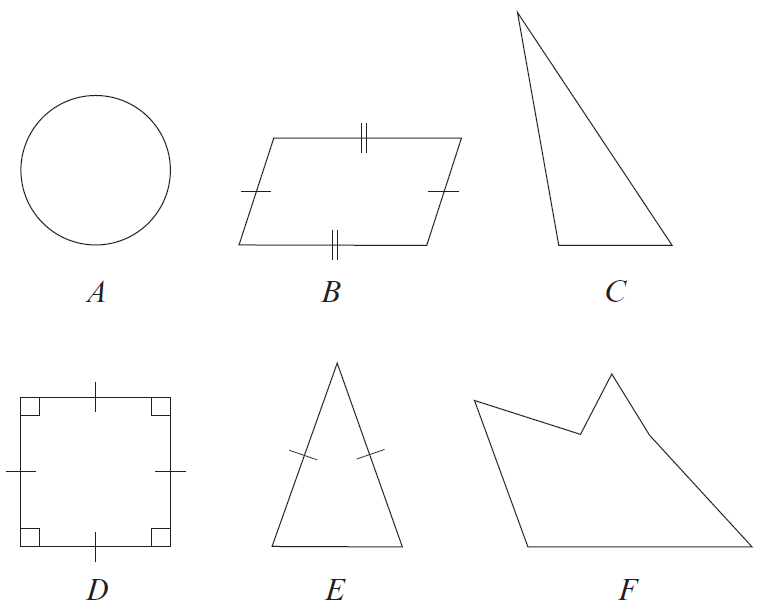
\includegraphics[width=10cm]{pictures/kpl3_2_teht7}
	\end{center}%
	\begin{vastaus}
		\alakohdat{
			§ $\{A, D, E\}$
			§ $\{A, B, D\}$
			§ $\{C, F\}$
			§ $\{A, D\}$
		}
	\end{vastaus}
\end{tehtava}

\begin{tehtava}
	Ratkaise avoin lause $4x^2 + 7x - 2 = 0$, kun perusjoukko
	on a) reaalilukujen joukko b) kokonaislukujen joukko.%
	\begin{vastaus}
		\alakohdat{
			§ $\{-2, \frac{1}{4}\}$
			§ $\{-2\}$
		}
	\end{vastaus}
\end{tehtava}

\begin{tehtava}
	Olkoot perusjoukko $\{ 0, 1, 2, \ldots , 10\}$, $A(x)$
	avoin lause ''$x \le 1$'' ja $B(x)$ avoin lause ''$x > 5$''.
	Ratkaise avoin lause.
	\alakohdat{
	§ $A(x)$,
	§ $\lnot B(x)$,
	§ $A(x) \land B(x)$,
	§ $\lnot A(x) \to B(x)$.
	}%
	\begin{vastaus}
		\alakohdat{
			§ $\{0, 1\}$
			§ $\{0, 1, 2, 3, 4 ,5\}$
			§ $\emptyset$
			§ $\{6, 7, 8, 9, 10\}$
		}
	\end{vastaus}
\end{tehtava}

\begin{tehtava}
	Arvotaan kaksi lukua, joista molemmat voivat olla 1, 2 tai 3. Arvonnan tuloksena saadaan lukupari $(x, y)$, missä $x$ on ensimmäisen arvonnan tulos ja $y$ toisen arvonnan tulos. Olkoot avoimet lauseet $S(x, y)$: ''$x \le y$'' ja $T(x, y)$: ''tulo $xy$ on jaollinen luvulla 3''. Ratkaise avoin lause, kun perusjoukon muodostavat arvonnan tuloksena saatavat mahdolliset lukuparit
	\[
	(1, 1),\ (1, 2),\ (1, 3),\ (2, 1),\ (2, 2),\ (2, 3),\ (3, 1),\ (3, 2),\ (3, 3).
	\]
	\alakohdat{
	§ $S(x, y)$,
	§ $\lnot T(x, y)$,
	§ $\lnot (S(x, y) \lor T(x, y))$,
	§ $S(x, y) \to T(x, y)$.
	}%
	\begin{vastaus}
		\alakohdat{
			§ $\{(1, 1), (1, 2), (1, 3), (2, 2), (2, 3), (3, 3)\}$
			§ $\{(1, 1), (1, 2), (2, 1), (2, 2)\}$
			§ $\{(2, 1)\}$
			§ $\{(1, 3), (2, 1), (2, 3), (3, 1), (3, 2), (3, 3)\}$
		}
	\end{vastaus}
\end{tehtava}

\begin{tehtava}
	Ratkaise reaalilukujen joukossa
	\alakohdat{
	§ epäyhtälö $x^2 \le 4$,
	§ epäyhtälöpari
	\[
	\left\{
	\begin{array}{rcl}
	x^2 & \le & 4 \\
	x & > & -1.
	\end{array}\right.
	\]
	}%
	\begin{vastaus}
		\alakohdat{
			§ $-2 \le x \le 2$
			§ $-1 < x \le 2$
		}
	\end{vastaus}
\end{tehtava}

\begin{tehtava}
	Ratkaise reaalilukujen joukossa epäyhtälö
	\alakohdat{
	§ $|x| > 5$,
	§ $|x| \le 1$,
	§ $|x - 4| > 5$,
	§ $|2x - 6| \le 1$.
	}%
	\begin{vastaus}
		\alakohdat{
			§ $(x < -5) \lor (x > 5)$
			§ $-1 \le x \le 1$
			§ $(-1 < x) \lor (x > 9)$
			§ $2,5 \le x \le 3,5$
		}
	\end{vastaus}
\end{tehtava}

\begin{tehtava}
	Ratkaise avoin lause reaalilukujen joukossa. Ilmaise ratkaisujoukko myös välimerkintää käyttäen.
	\alakohdat{
	§ $(x^2 > 1) \lor (0 \le x \le 2)$,
	§ $(x^2 > 1) \land (0 \le x \le 2)$,
	§ $(x^2 > 1) \to (0 \le x \le 2)$.
	}%
	\begin{vastaus}
		\alakohdat{
			§ $(x < -1) \lor (x \ge 0)$
			§ $1 < x \le 2$
			§ $-1 < x \le 2$
		}
	\end{vastaus}
\end{tehtava}

\begin{tehtava}
	Olkoot $P(x)$ avoin lause $(x < 10) \land (x^2 = 100)$ ja
	$Q(x)$ avoin lause $(x \ge 10) \lequiv (x^2 = 100)$. Ratkaise avoin lause reaalilukujen joukossa.
	\alakohdat{
	§ $P(x)$,
	§ $Q(x)$,
	§ $P(x) \lor Q(x)$,
	§ $P(x) \land Q(x)$.
	}%
	\begin{vastaus}
		\alakohdat{
			§ $x = -10$
			§ $(x \le 10) \land (x \ne -10)$
			§ $x \le 10$
			§ $\emptyset$
		}
	\end{vastaus}
\end{tehtava}

\end{tehtavasivu}

% -----


\begin{kotitehtavasivu}

\begin{tehtava}
	Olkoon $T(x, y)$ avoin lause ''$x$ lähettää tekstiviestin
	$y$:lle''. Suomenna lause.
	\alakohdat{
	§ $T(\textrm{Tiina}, \textrm{Elias})$,
	§ $\lnot T(\textrm{Elias}, \textrm{Tiina}) \land T(\textrm{Elias}, \textrm{Vilma})$,
	§ $T(x, x)$,
	§ $T(y, \textrm{Rasmus}) \lequiv T(\textrm{Rasmus}, y)$.
	}%
	\begin{vastaus}
		\alakohdat{
			§ Tiina lähettää tekstiviestin Eliakselle.
			§ Elias ei lähetä tekstiviestiä Tiinalle ja Elias lähettää tekstiviestin Vilmalle.
			§ $x$ lähettää tekstiviestin itselleen.
			§ $y$ lähettää Rasmukselle tekstiviestin jos ja vain jos Rasmus lähettää $y$:lle tekstiviestin.
		}
	\end{vastaus}
\end{tehtava}

\begin{tehtava}
	Olkoot $E(x)$ avoin lause ''$x$ on eurooppalainen
	pääkaupunki'' ja $S(x)$ avoin lause ''$x$ on suomalainen
	kaupunki''. Ratkaise avoin lause, kun perusjoukko on
	$\{\textrm{Helsinki}, \textrm{Rovaniemi}, \textrm{Praha}, \textrm{Milano}\}$.
	\alakohdat{
	§ $E(x)$,
	§ $\lnot S(x)$,
	§ $S(x) \land \lnot E(x)$,
	§ $\lnot (E(x) \land S(x))$,
	§ $E(x) \lequiv S(x)$.
	}%
	\begin{vastaus}
		\alakohdat{
			§ $\{\textrm{Helsinki}, \textrm{Praha}\}$
			§ $\{\textrm{Praha}, \textrm{Milano}\}$
			§ $\{\textrm{Rovaniemi}\}$
			§ $\{\textrm{Rovaniemi}, \textrm{Praha}, \textrm{Milano}\}$
			§ $\{\textrm{Helsinki}, \textrm{Milano}\}$
		}
	\end{vastaus}
\end{tehtava}

\begin{tehtava}
	Olkoon $R(x)$ avoin lause ''$x^2 - 100 > 0$''. Onko lause
	a) $R(10)$ b) $R(-15)$ tosi?%
	\begin{vastaus}
		\alakohdat{
			§ Ei.
			§ On.
		}
	\end{vastaus}
\end{tehtava}

\begin{tehtava}
	Olkoon $S(x, y)$ avoin lause ''$x^2 + y^2 = 5$''. Onko
	lause a) $S(2, 3)$ b) $S(2, -1)$ c) $S(-\sqrt{5}, 0)$ d)
	$S(-1, -1)$ tosi?%
	\begin{vastaus}
		\alakohdat{
			§ Ei.
			§ On.
			§ On.
			§ On.
		}
	\end{vastaus}
\end{tehtava}

\begin{tehtava}
	Ratkaise avoin lause $9x^2 + 30x + 25 \le 0$, kun
	määrittelyjoukko on a) reaalilukujen joukko b)
	kokonaislukujen joukko.%
	\begin{vastaus}
		\alakohdat{
			§ $x = -\frac{5}{3}$
			§ $\emptyset$
		}
	\end{vastaus}
\end{tehtava}

\begin{tehtava}
	Olkoot perusjoukko $\{ 1, 2, 3, \ldots , 16\}$, $C(x)$
	avoin lause ''luku 12 on jaollinen luvulla $x$'' ja $D(x)$ avoin lause ''luvun $x$ neliöjuuri on kokonaisluku''.
	Ratkaise avoin lause.
	\alakohdat{
	§ $C(x)$,
	§ $D(x)$,
	§ $\lnot C(x) \land D(x)$,
	§ $C(x) \lequiv D(x)$.
	}%
	\begin{vastaus}
		\alakohdat{
			§ $\{1, 2, 3, 4, 6, 12\}$
			§ $\{1, 4, 9, 16\}$
			§ $\{9, 16\}$
			§ $\{1, 4, 5, 7, 8, 10, 11, 13, 14, 15\}$
		}
	\end{vastaus}
\end{tehtava}

\begin{tehtava}
	Arvotaan kolme lukua, joista jokainen voi olla 1 tai
	2. Arvonnan tuloksena saadaan lukukolmikko $(x, y, z)$, missä $x$ on ensimmäisen arvonnan tulos, $y$ toisen arvonnan tulos ja $z$ kolmannen arvonnan tulos. Olkoot
	avoimet lauseet $S(x, y, z)$: ''$x + y + z \ge 5$'', $T(x,
	y, z)$: ''tulo $xyz$ on pariton'' ja $U(x, y, z)$: “summa
	$x + y + z$ on jaollinen luvulla 3''. Ratkaise avoin
	lause, kun perusjoukon muodostavat arvonnan tuloksena
	saatavat mahdolliset lukukolmikot
	\[
	(1, 1, 1),\ (1, 1, 2),\ (1, 2, 1),\ (1, 2, 2),\ (2, 1, 1),\ (2, 1, 2),\ (2, 2, 1),\ (2, 2, 2).
	\]
	\alakohdat{
	§ $S(x, y, z)$,
	§ $T(x, y, z)$,
	§ $U(x, y, z)$,
	§ $S(x, y, z) \land T(x, y, z)$,
	§ $S(x, y, z) \lor \lnot U(x, y, z)$,
	§ $\lnot (S(x, y, z) \lor T(x, y, z) \lor U(x, y, z))$,
	§ $S(x, y, z) \land (T(x, y, z) \lequiv U(x, y, z))$.
	}%
	\begin{vastaus}
		\alakohdat{
			§ $\{(1, 2, 2), (2, 1, 2), (2, 2, 1), (2, 2, 2)\}$
			§ $\{(1, 1, 1)\}$
			§ $\{(1, 1, 1), (2, 2, 2)\}$
			§ $\emptyset$
			§ $\{(1, 1, 2), (1, 2, 1), (1, 2, 2), (2, 1, 1), (2, 1, 2), (2, 2, 1), (2, 2, 2)\}$
			§ $\{(1, 1, 2), (1, 2, 1), (2, 1, 1)\}$
			§ $\{(1, 1, 2), (1, 2, 1), (1, 2, 2), (2, 1, 1), (2, 1, 2), (2, 2, 1)\}$
		}
	\end{vastaus}
\end{tehtava}

\begin{tehtava}
	Ratkaise reaalilukujen joukossa.
	\alakohdat{
	§ $(x^2 = 1) \lor (x(x + 5)(x - 1) = 0)$
	§ $(x^2 = 1) \land (x(x + 5)(x - 1) = 0)$
	}%
	\begin{vastaus}
		\alakohdat{
			§ $(x = -5) \lor (x = -1) \lor (x = 0) \lor (x = 1)$
			§ $x = 1$
		}
	\end{vastaus}
\end{tehtava}

\begin{tehtava}
	Ratkaise reaalilukujen joukossa
	\alakohdat{
	§ epäyhtälö $x^2 - 11x + 30 > 0$,
	§ epäyhtälöpari
	\[
	\left\{
	\begin{array}{rcl}
	x^2 - 11x + 30 & > & 0 \\
	2x & > & -6 - x.
	\end{array}\right.
	\]
	}%
	\begin{vastaus}
		\alakohdat{
			§ $(x < 5) \lor (6 < x)$
			§ $(-2 < x < 5) \lor (6 < x)$
		}
	\end{vastaus}
\end{tehtava}

\begin{tehtava}
	Ratkaise avoin lause reaalilukujen joukossa. Ilmaise ratkaisujoukko myös välimerkintää käyttäen.
	\alakohdat{
	§ $(-4 < x) \lor (x < 8)$,
	§ $(-4 < x) \land (x < 8)$,
	§ $((-4 < x) \land (x < 8)) \land (-5 \le x \le -3)$,
	§ $(-4 < x) \lequiv (-5 \le x \le -3)$.
	}%
	\begin{vastaus}
		\alakohdat{
			§ $x \in \mathbb{R}, x \in {]-\infty, \infty[}$
			§ $-4 < x < 8, x \in {]-4, 8[}$
			§ $-4 < x \le -3, x \in {]-4, -3]}$
			§ $(x \le -5) \lor (-4 < x \le -3), (x \in {]-\infty, -5]} \lor (x \in {]-4, -3]})$
		}
	\end{vastaus}
\end{tehtava}

\begin{tehtava}
	Olkoot $A(x)$ avoin lause $(x \ge 0) \to (x \ge 20)$
	ja $B(x)$ avoin lause $\lnot ((x \le 0) \lor (x \ge 20))$. Ratkaise avoin lause reaalilukujen joukossa.
	\alakohdat{
	§ $A(x)$,
	§ $B(x)$,
	§ $A(x) \lor B(x)$.
	}
	\begin{vastaus}
		\alakohdat{
			§ $(x < 0) \lor (x \ge 20)$
			§ $0 < x < 20$
			§ $x \in \mathbb{R} \setminus \{0\} \Leftrightarrow x \ne 0$
		}
	\end{vastaus}
\end{tehtava}

\end{kotitehtavasivu}
